\documentclass[10pt,twocolumn]{article}

\usepackage[letterpaper,top=0.68in,bottom=0.68in,left=0.58in,right=0.58in,columnsep=0.28in]{geometry}
\usepackage[T1]{fontenc}
\usepackage[utf8]{inputenc}
\usepackage{lmodern}
\usepackage{microtype}
\usepackage{xcolor}
\usepackage{amsmath,amssymb}
\usepackage{booktabs,tabularx,array}
\usepackage{enumitem}
\usepackage{listings}
\usepackage[most]{tcolorbox}
\usepackage{tikz}
\usetikzlibrary{arrows.meta,positioning,calc,fit}
\usepackage{titlesec}
\usepackage{fancyhdr}
\usepackage[hidelinks]{hyperref}
\usepackage{ragged2e}

\hypersetup{
  pdftitle={How an Approved Candidate Reaches main},
  pdfsubject={Candidate commits, landing commits, and safe Git integration},
  pdfauthor={CoCoA SONIC maintainers}
}

% The guide uses the same restrained visual language for concepts, safe
% states, cautions, and refusal states on every page.
\definecolor{ink}{HTML}{18202A}
\definecolor{muted}{HTML}{5D6875}
\definecolor{rulegray}{HTML}{D8DEE5}
\definecolor{panel}{HTML}{F3F6F8}
\definecolor{blue}{HTML}{235C8E}
\definecolor{bluepale}{HTML}{EAF2F8}
\definecolor{green}{HTML}{2F6E4E}
\definecolor{greenpale}{HTML}{EAF4EE}
\definecolor{amber}{HTML}{8A5A00}
\definecolor{amberpale}{HTML}{FFF5D9}
\definecolor{red}{HTML}{8B2F36}
\definecolor{redpale}{HTML}{FBEAEC}
\definecolor{codebg}{HTML}{F5F7F9}

\color{ink}
\setlength{\parindent}{0pt}
\setlength{\parskip}{3.5pt}
\setlist[itemize]{leftmargin=1.15em,itemsep=1.5pt,topsep=2pt}
\setlist[enumerate]{leftmargin=1.25em,itemsep=1.5pt,topsep=2pt}
\setlength{\emergencystretch}{2em}
\raggedbottom

\titleformat{\section}
  {\large\bfseries\color{blue}}
  {\thesection}{0.45em}{}
\titlespacing*{\section}{0pt}{9pt}{3pt}

\titleformat{\subsection}
  {\normalsize\bfseries\color{ink}}
  {\thesubsection}{0.4em}{}
\titlespacing*{\subsection}{0pt}{7pt}{2pt}

\lstdefinestyle{shell}{
  backgroundcolor=\color{codebg},
  basicstyle=\ttfamily\footnotesize,
  columns=fullflexible,
  keepspaces=true,
  showstringspaces=false,
  breaklines=true,
  frame=single,
  rulecolor=\color{rulegray},
  framerule=0.5pt,
  xleftmargin=3pt,
  xrightmargin=3pt,
  aboveskip=4pt,
  belowskip=4pt
}
\lstset{style=shell}

\newtcolorbox{metabox}{
  enhanced,
  colback=panel,
  colframe=rulegray,
  boxrule=0.6pt,
  arc=1.5mm,
  left=2.5mm,right=2.5mm,top=1.8mm,bottom=1.8mm
}

\newtcolorbox{summarybox}[1][]{
  enhanced,
  colback=bluepale,
  colframe=blue,
  boxrule=0.7pt,
  arc=1.5mm,
  left=2mm,right=2mm,top=1.4mm,bottom=1.4mm,
  fonttitle=\bfseries,
  title=#1
}

\newtcolorbox{keybox}[1][]{
  enhanced,
  colback=greenpale,
  colframe=green,
  boxrule=0.7pt,
  arc=1.5mm,
  left=2mm,right=2mm,top=1.4mm,bottom=1.4mm,
  fonttitle=\bfseries,
  title=#1
}

\newtcolorbox{warningbox}[1][]{
  enhanced,
  colback=amberpale,
  colframe=amber,
  boxrule=0.7pt,
  arc=1.5mm,
  left=2mm,right=2mm,top=1.4mm,bottom=1.4mm,
  fonttitle=\bfseries,
  title=#1
}

\newtcolorbox{stopbox}[1][]{
  enhanced,
  colback=redpale,
  colframe=red,
  boxrule=0.7pt,
  arc=1.5mm,
  left=2mm,right=2mm,top=1.4mm,bottom=1.4mm,
  fonttitle=\bfseries,
  title=#1
}

\setlength{\headheight}{19pt}
\pagestyle{fancy}
\fancyhf{}
\fancyhead[L]{\footnotesize\color{muted}AI-assisted coding workflow}
\fancyhead[R]{\footnotesize\color{muted}Candidate $C$ to landing $L$}
\fancyfoot[C]{\footnotesize\color{muted}\thepage}
\renewcommand{\headrulewidth}{0.4pt}
\renewcommand{\headrule}{\hbox to\headwidth{\color{rulegray}\leaders\hrule height \headrulewidth\hfill}}

\newcommand{\code}[1]{\texttt{#1}}
\newcommand{\term}[1]{\textbf{#1}}

\begin{document}

\twocolumn[
\begin{@twocolumnfalse}
\vspace*{-0.24in}
{\sffamily\bfseries\fontsize{20}{23}\selectfont\color{ink}
How an Approved Candidate Reaches \texttt{main}\par}
\vspace{4pt}
{\sffamily\large\color{blue}
Understanding candidate $C$, landing $L$, Git tree objects, and the watcher operations that connect them\par}
\vspace{7pt}
\begin{metabox}
\small
\begin{tabularx}{\textwidth}{>{\bfseries}p{0.13\textwidth} X >{\bfseries}p{0.11\textwidth} X}
Purpose & Explain the landing mechanism for a reader who normally uses commits, branches, merges, and pull requests. & Audience & Students, users, and maintainers of the AI-assisted coding ticket system.\\
Key rule & The Architect approves exact candidate $C$. The watcher calculates, verifies, and records distinct landing $L$. & Scope & Git objects, the three central commands, safe local landing, recovery, and remote publication.\\
\end{tabularx}
\end{metabox}
\vspace{5pt}
\end{@twocolumnfalse}
]

\begin{summarybox}[Executive summary]
The Implementer creates immutable candidate commit $C$. The Architect audits
that exact commit and either approves or rejects it. After approval, the
watcher---the running \code{mailbox\_daemon.py} program---combines the approved
candidate change with current local \code{main}, creates distinct
single-parent landing commit $L$, and verifies its Git objects and safe
checkout conditions. The watcher then fast-forwards local \code{main}. It
attempts one ordinary, non-force push and records a recovery instruction if
the remote cannot be verified.
\end{summarybox}

\begin{warningbox}[These are internal operations]
The command fragments below explain what the watcher does. A user does not
run them to land a ticket. The watcher owns landing, recovery records, and the
safe update of \code{main}.
\end{warningbox}

\section{The five objects to keep separate}

\begin{tabularx}{\columnwidth}{>{\bfseries}p{0.10\columnwidth} X}
$B$ & The saved version from which the ticket began.\\
$C$ & The exact candidate commit produced by the Implementer and audited by the Architect.\\
$M$ & The exact commit at the tip of local \code{main} when landing is prepared.\\
$T$ & A Git \emph{tree object}: the complete repository snapshot obtained by combining $M$ with the approved change represented by $C$.\\
$L$ & The new landing commit. It points to snapshot $T$ and has $M$ as its sole parent.\\
\end{tabularx}

\begin{keybox}[One-sentence mental model]
$C$ is what the Architect approved; $T$ is the integrated repository
snapshot; $L$ records that snapshot as the next commit after current local
\code{main} $M$.
\end{keybox}

\section{Why the word ``tree'' is confusing}

Git uses \term{tree} in a narrower sense than ordinary conversation. Three
related ideas are often mixed together:

\begin{enumerate}
  \item A \term{directory tree}: folders and files on disk.
  \item A \term{commit graph}: commits connected by parent relationships.
  \item A Git \term{tree object}: Git's stored description of one directory snapshot.
\end{enumerate}

In \code{git commit-tree} and \code{git merge-tree}, the important meaning is
number 3.

\subsection{A Git commit does not directly contain files}

A commit points to a root tree object. That tree lists filenames and points
to either file contents, called \term{blobs}, or more tree objects that
represent subdirectories.

\begin{center}
\begin{tikzpicture}[
  node distance=5mm and 7mm,
  every node/.style={font=\scriptsize,align=center},
  box/.style={draw=rulegray,rounded corners=1mm,fill=panel,inner sep=3pt},
  obj/.style={draw=blue,rounded corners=1mm,fill=bluepale,inner sep=3pt},
  arr/.style={-{Latex[length=1.7mm]},thick,color=muted}
]
\node[obj] (commit) {commit $L$\\parent: $M$\\tree: $T$};
\node[obj,below=of commit] (tree) {tree $T$\\root directory};
\node[box,below left=of tree] (blob1) {blob\\\texttt{README.md}};
\node[box,below right=of tree] (subtree) {tree\\\texttt{src/}};
\node[box,below=of subtree] (blob2) {blob\\\texttt{model.py}};
\draw[arr] (commit) -- node[right]{snapshot} (tree);
\draw[arr] (tree) -- (blob1);
\draw[arr] (tree) -- (subtree);
\draw[arr] (subtree) -- (blob2);
\end{tikzpicture}
\end{center}

The root tree $T$ means:

\begin{quote}
``Here is the complete set of filenames, directories, permissions, and file
contents for this version of the repository.''
\end{quote}

It does \emph{not} mean a branch, a checked-out folder, or a history graph.

\section{Candidate \texorpdfstring{$C$}{C} versus landing \texorpdfstring{$L$}{L}}

Suppose the candidate started from $B$. While it was being developed,
another accepted ticket advanced local \code{main} to $M$:

\begin{center}
\begin{tikzpicture}[
  x=12mm,y=8mm,
  every node/.style={font=\scriptsize},
  commit/.style={circle,draw=ink,fill=white,minimum size=4.5mm,inner sep=0pt},
  label/.style={font=\scriptsize,align=left},
  line/.style={thick,color=muted}
]
\node[commit] (B) at (0,0) {$B$};
\node[commit] (M) at (2,0) {$M$};
\node[commit] (C) at (2,1.25) {$C$};
\draw[line] (B)--(M);
\draw[line] (B)--(C);
\node[label,right=2mm of M] {current local \texttt{main}};
\node[label,right=2mm of C] {approved candidate};
\end{tikzpicture}
\end{center}

The watcher must preserve all accepted work already in $M$ and the approved
change from the $B\rightarrow C$ side. It creates a linear commit $L$ after
$M$:

\begin{center}
\begin{tikzpicture}[
  x=11mm,y=8mm,
  every node/.style={font=\scriptsize},
  commit/.style={circle,draw=ink,fill=white,minimum size=4.5mm,inner sep=0pt},
  landing/.style={circle,draw=green,fill=greenpale,minimum size=5.2mm,inner sep=0pt},
  label/.style={font=\scriptsize,align=left},
  line/.style={thick,color=muted}
]
\node[commit] (B) at (0,0) {$B$};
\node[commit] (M) at (2,0) {$M$};
\node[landing] (L) at (4,0) {$L$};
\node[commit] (C) at (2,1.25) {$C$};
\draw[line] (B)--(M)--(L);
\draw[line] (B)--(C);
\node[label,right=2mm of C] {audited object};
\node[label,right=2mm of L] {integrated commit\\on local \texttt{main}};
\end{tikzpicture}
\end{center}

$C$ and $L$ are distinct commits. A commit hash depends on its parent,
message, author and committer metadata, timestamp, and root tree. $L$ has
parent $M$ and a recovery-bound message, so the watcher rejects any record
that tries to use $C$ itself as $L$.

\section{The three central Git commands}

The following shell-shaped transcription makes the data flow visible. The
Python watcher passes the landing message to \code{commit-tree} directly
rather than launching this shell pipeline.

\begin{lstlisting}
M=$(git rev-parse --verify \
      'refs/heads/main^{commit}')

T=$(git merge-tree --write-tree "$M" "$C")

L=$(printf '%s' "$LANDING_MESSAGE" | \
      git commit-tree "$T" -p "$M" -F -)
\end{lstlisting}

The notation \code{X=\$(command)} means: run \code{command}, capture the text
it prints, and store that text in variable \code{X}.

\subsection{Command 1: freeze current local main}

\begin{lstlisting}
M=$(git rev-parse --verify \
      'refs/heads/main^{commit}')
\end{lstlisting}

\code{refs/heads/main} is Git's full internal name for the local branch
\code{main}. A branch name is movable; it points to a commit. The
\code{\^\{commit\}} suffix requires that the result be a commit, and
\code{--verify} refuses an invalid name.

The command asks: ``What exact commit does local \code{main} point to?'' It
may print:

\begin{lstlisting}
a7f83011c38cb4e91e453a137efab5f727d91631
\end{lstlisting}

That immutable hash is stored in $M$. No file, branch, or commit changes.

\begin{keybox}[Why record $M$?]
\code{main} is a moving label. $M$ is a fixed object. The landing operation
can prove exactly which version it used as the parent.
\end{keybox}

\subsection{Command 2: compute the integrated snapshot}

\begin{lstlisting}
T=$(git merge-tree --write-tree "$M" "$C")
\end{lstlisting}

\code{git merge-tree} invokes Git's three-way merge machinery. Git finds a
common ancestor and compares both sides:

\begin{align*}
B &\rightarrow M && \text{changes already on main},\\
B &\rightarrow C && \text{approved candidate changes}.
\end{align*}

\code{--write-tree} stores the successfully combined repository snapshot as
a new tree object and prints its hash. At this point Git has created only a
snapshot object. It has not created a commit, moved a branch, staged a file,
or modified a checkout.

\begin{warningbox}[This still uses Git's merge algorithm]
The workflow avoids a conventional checked-out \code{git merge} and a
two-parent merge commit. It does not avoid merge logic. \code{merge-tree}
calculates the integrated file contents.
\end{warningbox}

\subsection{What happens on a conflict?}

Suppose both sides change the same line incompatibly:

\begin{lstlisting}
# At common base B
learning_rate = 0.001

# At current local main M
learning_rate = 0.0005

# At candidate C
learning_rate = 0.01
\end{lstlisting}

Git cannot determine which value is correct. \code{merge-tree} reports
failure, and the watcher stops.

\begin{stopbox}[Why stopping is correct]
Automatic conflict resolution would create code different from candidate $C$
that the Architect audited. The conflict requires new implementation and a
new audit rather than an unreviewed repair during landing.
\end{stopbox}

\subsection{Command 3: create the landing commit}

\begin{lstlisting}
L=$(printf '%s' "$LANDING_MESSAGE" | \
      git commit-tree "$T" -p "$M" -F -)
\end{lstlisting}

\code{git commit-tree} creates a commit directly from Git objects:

\begin{tabularx}{\columnwidth}{>{\ttfamily}p{0.22\columnwidth} X}
\$T & The complete repository snapshot for the new commit.\\
-p \$M & The new commit's sole parent is $M$.\\
-F - & Read the complete commit message from standard input.\\
\end{tabularx}

The watcher does not invent a generic landing message. It copies the complete
human-readable message already stored in approved candidate $C$, then appends
two machine-readable recovery lines:

\begin{lstlisting}
Mailbox-Cycle: EXACT-CYCLE-ID
Mailbox-Candidate: FULL-CANDIDATE-COMMIT
\end{lstlisting}

Those lines bind $L$ to the ticket cycle and exact candidate that the
Architect approved. \code{commit-tree} prints the new commit hash, which is
stored in $L$.

\begin{keybox}[Why $L$ is not a merge commit]
A merge commit has two or more parents. $L$ has exactly one parent, $M$. Its
snapshot contains the integrated files, but the history of \code{main}
remains linear.
\end{keybox}

\section{Why no checkout or staging is needed}

Most everyday Git commands operate through three layers:

\begin{enumerate}
  \item the working directory;
  \item the staging area, also called the index;
  \item the Git object database.
\end{enumerate}

The familiar sequence

\begin{lstlisting}
git add file.py
git commit -m "message"
\end{lstlisting}

reads files from the working directory, places their desired state in the
index, and then creates tree and commit objects. The watcher already knows
exact tree $T$, so it can create $L$ without using the working directory or
index:

\begin{center}
\begin{tikzpicture}[
  node distance=5mm,
  every node/.style={font=\scriptsize,align=center},
  normal/.style={draw=rulegray,rounded corners=1mm,fill=panel,minimum width=24mm,inner sep=3pt},
  direct/.style={draw=green,rounded corners=1mm,fill=greenpale,minimum width=24mm,inner sep=3pt},
  arr/.style={-{Latex[length=1.7mm]},thick,color=muted}
]
\node[normal] (wd) {working\\directory};
\node[normal,right=of wd] (idx) {staging area\\index};
\node[normal,right=of idx] (obj) {tree and\\commit objects};
\draw[arr] (wd)--(idx);
\draw[arr] (idx)--(obj);
\node[direct,below=7mm of idx] (watcher) {watcher already\\has tree $T$};
\draw[arr] (watcher)--(obj);
\end{tikzpicture}
\end{center}

Constructing $L$ therefore does not touch the user's files. Updating the
user's folder is a later, separately checked step.

\section{A complete worked example}

Assume common base $B$ contains:

\begin{lstlisting}
src/model.py
tests/test_model.py
\end{lstlisting}

Candidate $C$ modifies both files. Another accepted ticket advances
\code{main} to $M$ by adding:

\begin{lstlisting}
src/logging.py
\end{lstlisting}

\code{merge-tree} calculates $T$ with all three desired files:

\begin{lstlisting}
src/logging.py       # retained from M
src/model.py         # candidate version from C
tests/test_model.py  # candidate version from C
\end{lstlisting}

\code{commit-tree} records that snapshot as $L$ with parent $M$:

\begin{center}
\begin{tikzpicture}[
  x=10mm,y=8mm,
  every node/.style={font=\scriptsize},
  commit/.style={circle,draw=ink,fill=white,minimum size=4.5mm,inner sep=0pt},
  landing/.style={circle,draw=green,fill=greenpale,minimum size=5.2mm,inner sep=0pt},
  line/.style={thick,color=muted}
]
\node[commit] (B) at (0,0) {$B$};
\node[commit] (M) at (2,0) {$M$};
\node[landing] (L) at (4,0) {$L$};
\node[commit] (C) at (2,1.2) {$C$};
\draw[line] (B)--(M)--(L);
\draw[line] (B)--(C);
\end{tikzpicture}
\end{center}

\code{git diff M L} contains only the approved candidate delta. The
\code{logging.py} addition is already present in both $M$ and $L$, so it does
not appear as a new change in that comparison.

\section{Why not use ordinary merge or cherry-pick?}

\subsection{Ordinary merge}

A conventional merge may create a commit with both $M$ and $C$ as parents.
That would preserve the candidate branch topology in \code{main}. This
workflow wants one linear landing commit for one accepted ticket.

\subsection{Cherry-pick}

Cherry-pick naturally applies one or more commits. Candidate development may
contain several intermediate commits:

\begin{center}
$B\rightarrow c_1\rightarrow c_2\rightarrow C$
\end{center}

The landing rule records their net result as one commit after $M$.
\code{merge-tree} plus \code{commit-tree} computes the complete branch result
without replaying each intermediate implementation commit into \code{main}.

\section{How the watcher verifies and records landing L}

Creating $L$ does not immediately move \code{main}. The watcher first:

\begin{enumerate}
  \item saves $L$ under a private Git reference and checks that the reference points to exact $L$;
  \item checks that $L$ has exactly one parent, $M$;
  \item recalculates the expected squash tree and compares it with $L$'s tree; and
  \item checks that $L$'s message exactly preserves $C$'s approved message and the two recovery lines.
\end{enumerate}

These are Git identity and recovery checks. They do \emph{not} rerun the
ticket's scientific tests or gates on $L$. The Architect already audited the
test evidence for exact candidate $C$.

\begin{warningbox}[Why the private reference matters]
A new Git object can become hard to recover if no branch or reference points
to it. The private landing reference preserves exact $L$ before the user's
branch changes. A restart verifies and reuses that object instead of silently
building a different landing.
\end{warningbox}

\section{When does local main move?}

The user's main folder must pass every condition below:

\begin{itemize}
  \item Git has the folder attached to local branch \code{main};
  \item local \code{main} still points to parent $M$ used to build $L$; and
  \item the folder has no staged, unstaged, or untracked files.
\end{itemize}

Only then does the watcher run the equivalent of:

\begin{lstlisting}
git merge --ff-only L
\end{lstlisting}

Because $L$ has $M$ as its direct parent, this command performs no new
content merge. It moves the branch and clean checkout from $M$ to $L$.

\begin{stopbox}[If the folder is not safe]
The watcher leaves the user's folder untouched and preserves candidate $C$,
Architect GO, and prepared landing $L$. Unfinished files require the user to
make the folder clean and restart. If \code{main} moved to another saved
commit after $L$ was prepared, candidate $C$ requires a new Architect audit.
\end{stopbox}

\section{Local landing and GitHub are separate}

Local \code{main} reaching $L$ completes the local landing. The watcher then
attempts one ordinary, non-force push of exact $L$ to remote
\code{origin/main} and checks that the remote reports that same commit.

If the push fails or the remote result cannot be verified, the watcher does
not rewrite history and does not repeat the ticket. Local $L$ remains
accepted. A file named
\code{pending-main-push-\textit{L}.txt} records the exact commit and command
still owed.

\begin{keybox}[Two separate questions]
``Did the ticket land locally?'' asks whether local \code{main} is exact $L$.
``Did GitHub receive it?'' asks whether \code{origin/main} is exact $L$. A
network or remote-branch problem can make the second answer no while the first
answer remains yes.
\end{keybox}

\section{Safety properties}

\begin{itemize}
  \item \term{Immutable audit target:} the Architect's decision names exact candidate $C$.
  \item \term{Distinct accepted object:} the watcher rejects any landing record that uses $C$ itself as $L$.
  \item \term{Current-main preservation:} $L$ is built after actual landing parent $M$.
  \item \term{Fail-closed conflicts:} incompatible concurrent changes stop landing.
  \item \term{Linear main history:} $L$ has one parent.
  \item \term{No role-owned integration:} the parent watcher, not Architect, Implementer, or Red Team, creates $L$ and updates \code{main}.
  \item \term{No hidden test claim:} object verification is not described as a new scientific test run.
  \item \term{Recoverable preparation:} a private reference preserves exact $L$ before the branch moves.
  \item \term{Protected remote history:} the watcher attempts no force push.
\end{itemize}

\section{Where the implementation lives}

The current source of truth is \path{ai/tools/mailbox_daemon.py}. These
functions divide the mechanism into reviewable steps:

\begin{tabularx}{\columnwidth}{>{\raggedright\arraybackslash}p{0.47\columnwidth} >{\raggedright\arraybackslash}X}
\toprule
\normalfont\bfseries Function & \bfseries Responsibility\\
\midrule
\path{_exact_squash_tree} & Calculate $T$ with \code{merge-tree}.\\
\path{_landing_commit_message} & Preserve $C$'s message and add recovery facts.\\
\path{prepare_exact_squash_landing} & Create, journal, and verify $L$.\\
\path{_verify_prepared_landing} & Recalculate parent, tree, and message checks.\\
\path{land_prepared_commit_in_clean_user_checkout} & Check the user's folder and fast-forward local \code{main}.\\
\path{push_exact_landing_or_record_debt} & Push once without force or save the owed action.\\
\bottomrule
\end{tabularx}

\section{Compact translation table}

\begin{tabularx}{\columnwidth}{>{\ttfamily\footnotesize}p{0.35\columnwidth} >{\raggedright\arraybackslash}X}
\toprule
\normalfont\bfseries Command or object & \bfseries Plain-English meaning\\
\midrule
C & Exact implementation approved by the Architect.\\
M & Exact current commit at local \texttt{main}.\\
T & Complete integrated snapshot stored as a Git tree object.\\
L & Distinct single-parent commit that records $T$ after $M$.\\
rev-parse & Resolve and verify a name as one exact commit.\\
merge-tree & Calculate merged file contents without a checkout-based merge.\\
--write-tree & Store the calculated snapshot and print its hash.\\
commit-tree & Create a commit directly from a tree object.\\
-p M & Declare $M$ as the new commit's parent.\\
-F - & Read the complete commit message from standard input.\\
--ff-only & Move \texttt{main} only when no new merge is required.\\
\bottomrule
\end{tabularx}

\begin{summarybox}[Final mental model]
\begin{enumerate}
  \item Freeze current local \code{main} as commit $M$.
  \item Calculate integrated snapshot $T$ from $M$ and approved candidate $C$.
  \item Create distinct landing $L$ with snapshot $T$ and sole parent $M$.
  \item Verify $L$'s parent, tree, message, and recovery reference.
  \item Check the user's \code{main} folder and fast-forward it from $M$ to $L$.
  \item Attempt one non-force push; record the exact owed command if the remote cannot be verified.
\end{enumerate}
\end{summarybox}

\end{document}
